\subsection{Discovery of Neutrinos}

\begin{figure}
\begin{center}
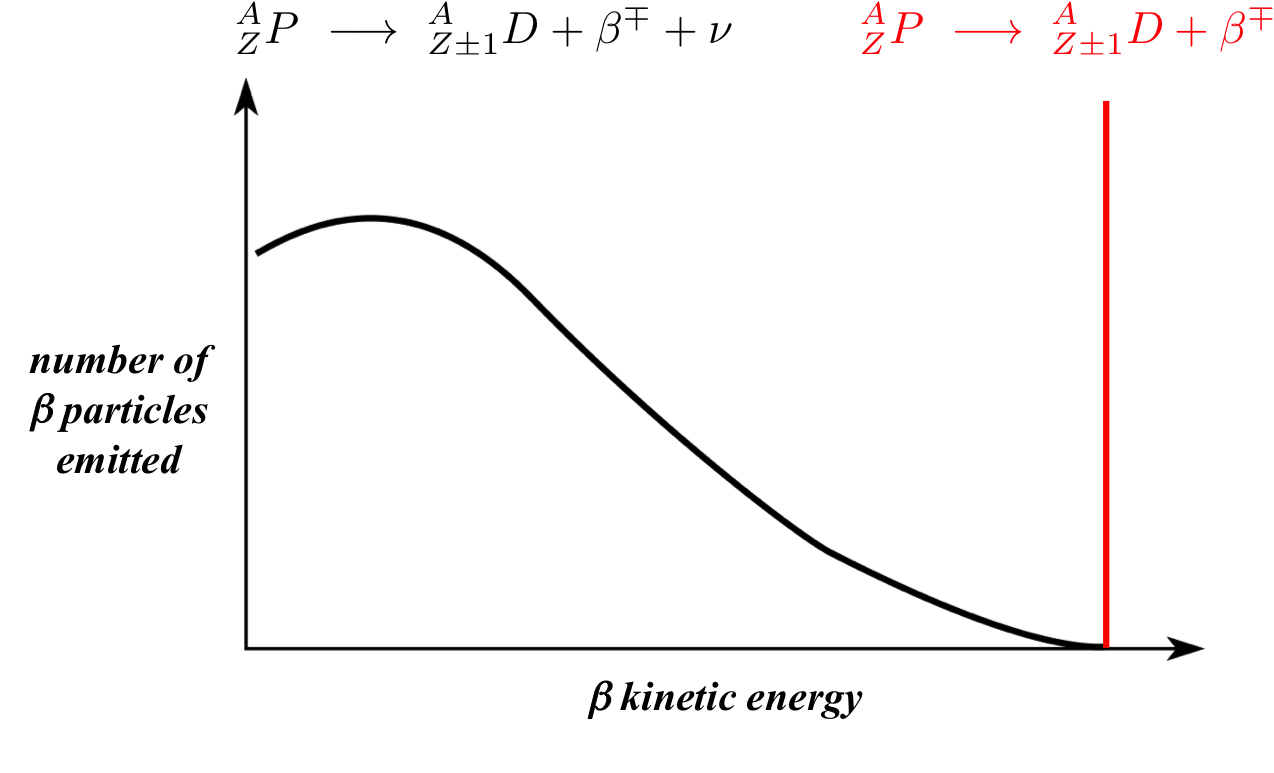
\includegraphics[width=0.75\columnwidth]{Neutrino/betaspectrum.png}
\caption{Kinetic energy distribution of the $\beta$ particle (electron or positron) produced in the decay of a parent nucleus $P$ into a daughter nucleus $D$. Units are arbitrary. Red curve: neutrinoless $\beta$ decay (Eq.~\ref{eq:beta_dirac}). The position of the quasi-Dirac spectrum is obtained by computing the reaction quotient. Black curve: continuous spectrum of $\beta$ decay involving a third particle (Eq.~\ref{eq:beta_cont}). Here, $\nu$ refers to an electron neutrino or antineutrino in the $\beta^{+}$ and $\beta^{-}$ decay respectively.}
\label{fig:betaspectrum}
\end{center}
\end{figure}

Two years following the discovery of the electron in 1897 by Sir Joseph John Thomson, Hernest Rutherford distinguished two types of radioactive emissions from some atomic nuclei: \textit{alpha} decay, where the nuclei emit $^{4}_2 \mathrm{He}^{2+}$; and \textit{beta} decay, in which the nuclei emit an electron\footnote{or a positron, differentiating between $\beta^{\mp}$ decays}. In 1914, however, it became apparent that an important ingredient was missing. In fact, if only a $\beta$ particle were released from the transmutation of a parent nucleus $P$ into a daughter nucleus $D$, \textit{i.e.}

\begin{equation}
\label{eq:beta_dirac}
\begin{array}{ccc}
^{A}_{Z}P & \longrightarrow & ^{A}_{Z\pm1}\mathrm{D}^{\pm} + \beta^{\mp}
\end{array}
\end{equation} \\ then the momentum spectrum of the beta particle would be a quasi-Dirac\footnote{because of Heisenberg's uncertainty principle, $\Delta E \Delta t \sim \hbar$, it would have some fundamental albeit tiny width due to the intrinsic uncertainty on the particle's energy} as illustrated by the red line in Fig.~\ref{fig:betaspectrum}. However, the momentum spectrum of the $\beta$ particles were instead continous, as per the black curve in  Fig.~\ref{fig:betaspectrum}. This suggests either that energy isn't conserved in $\beta$ decays or that the energy of the $\beta$ particle is shared by an additional unseen particle. This latter remedy, characterised as desperate at the time, was postulated by Wolfgang Pauli in 1930 in a famous letter\footnote{\url{http://www.physics.princeton.edu/~mcdonald/examples/EP/pauli_neutrino_30_english.pdf}} adressed to the community of \guillemotleft \textit{radioactive ladies and gentlemen} \guillemotright. He is often quoted saying to Niels Bohr: \\
\vspace{5pt}
\begin{center}
{\guillemotleft} ~I have done a terrible thing: I have postulated a particle that cannot be detected. ~ {\guillemotright} \\
\end{center}
\vspace{5pt}
Although many PhD students are often brought to make much more terrible assumptions, the existence of Pauli's undetectable particle was eventually inferred from weak interactions, the framework of which was developped by Enrico Fermi only 4 years later. In our current interpretation of $\beta$ decay, the transmutation of atomic nuclei is enabled by the emission or absorption of a $W^{\pm}$ gauge boson which mediates --- along with the $Z^0$ boson --- the weak interaction. These bosons are heavier than the nucleons they transmute which in turn make them, according to the Heisenberg uncertainty principle, very short-lived, with a half life of $\sim 3 \times 10^{-25}~s$. As such, this interaction is deemed short-ranged, hence coined \textit{weak} interaction. In the case of $\beta^{\mp}$ decay, the $W$ boson decays into an electron (or positron) and the additional particle, labelled $\nu$, such that
\begin{equation}
\label{eq:beta_cont}
\left\{
\begin{array}{lcl}
^{A}_{Z}P & \longrightarrow & ^{A}_{Z\pm1}\mathrm{D}^{\pm} + W^{\mp} \\
W^{\mp} & \longrightarrow & e^{\mp} + \nu
\end{array}
\right.
\end{equation} \\ whose properties were derived from Enrico Fermi's newly built theory of the weak interaction and dubbed the hypothetical particle the \textbf{neutrino} as it must be electrically neutral, and is very small\footnote{in the context of particle physics, small refers to its interaction cross section}. As it turns out, the particle involved in $\beta^{-}$ decay of neutrons is actually its conjugate anti-particle, the electron \textit{antineutrino}. Initially, neutrinos\footnote{technically speaking, neutrino borrowing of Italian vocabulary, the plural form should be \textbf{neutrini}. However, to prevent any confusion, I chose to use the anglocentric version, \textbf{neutrinos}} were thought to be massless and virtually undetectable. Nevertheless, neutrinos were discovered in 1956 when nuclear reactor synthesized antineutrinos by beta decay reacted with protons to produce neutrons and positrons \citep{nu_e_discovery}, a reaction known as \textit{electron capture} (see second expression in Eq.~\ref{eq:three_reactions}). The discovery is attributed to Clyde Cowan and Fredrick Reines who have been awarded the 1995 physics Nobel prize. In the following subsection, I summarize the neutrino's properties in the context of the standard model of particle physics.\\

\subsection{The Standard Model of Particle Physics}

\subsubsection{Neutral Leptons}

All fundamental particles are described by a set of quantum numbers, \textit{i.e.} degrees of freedom to fully determine their wave function. In addition to their principal ($n$), azimuthal ($\ell$) and magnetic ($m$) quantum numbers, the wave function of a fundamental particle requires the knowledge of its spin ($s$) which can either be an integer (bosons) or semi-integer (fermions) multiple of the Planck action $\hbar$. In the Standard Model (SM) of particle physics, fermions with $s/\hbar=1/2$ can be distinguished between two main types of particles: \\

\begin{itemize}
\item[$\bullet$] quarks, which are sensitive to all four fundamental interactions: strong, weak, electromagnetic and gravitational. They interact with one another via gluons, the carrier boson for the strong interaction. Due to color confinement, a property of the strong interaction, quarks cannot be observed directly in isolation, but rather through the composite particles they constitute:\\
\begin{itemize}
\item[$\star$] baryons, which have 3 valence quarks,\\
\item[$\star$] mesons, which are a combination of a quark and an antiquark. \\
\end{itemize}
These two can be distinguished by the computation of the baryon number $B = n_q - n_{\bar{q}}$ which is defined as the number of quarks (each having $n_q = 1/3$) minus the number of their conjugate anti-quarks ($n_q = -1/3$). As such, baryons have $B=1$ whereas mesons have $B=0$. There are 6 different quark flavours, \textit{a.k.a.} colours, arranged into 3 generations of hierarchical mass of a positively ($Q/e=2/3$) and a negatively ($Q/e=-1/3$) charged pair:\\
\begin{itemize}
\item[$\star$] first (light) generation: \textit{up} ($u$) and \textit{down} ($d$), \\
\item[$\star$] second (medium) generation: \textit{charm} ($c$) and \textit{strange} ($s$), \\
\item[$\star$] third (heavy) generation: \textit{top} ($t$) and \textit{bottom} ($b$). \\
\end{itemize}

\item[$\bullet$] leptons, which are not sensitive to the strong interaction, and, in the case of neutrinos, the electromagnetic interaction. There are 6 different leptons, arranged into 3 generations of hierarchical mass\footnote{this is not necessarily the case for the neutrinos} of a negatively charged ($Q/e=-1$) and electrically neutral pair: \\
\begin{itemize}
\item[$\star$] first (electronic) generation: $e$ and $\nu_e$, \\
\item[$\star$] second (muonic) generation: $\mu$ and $\nu_\mu$, \\
\item[$\star$] third (tauic) generation: $\tau$ and $\nu_\tau$, \\
\end{itemize}
Leptons are characterized by a lepton number, which is $L=1$ for any lepton and $L=-1$ for any anti-lepton. \\
\end{itemize}

\subsubsection{The Weak Interaction}

\begin{figure}
\begin{center}
%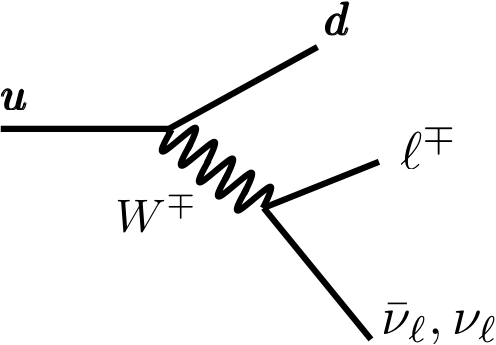
\includegraphics[width=0.35\columnwidth]{Neutrino/bcci.png}
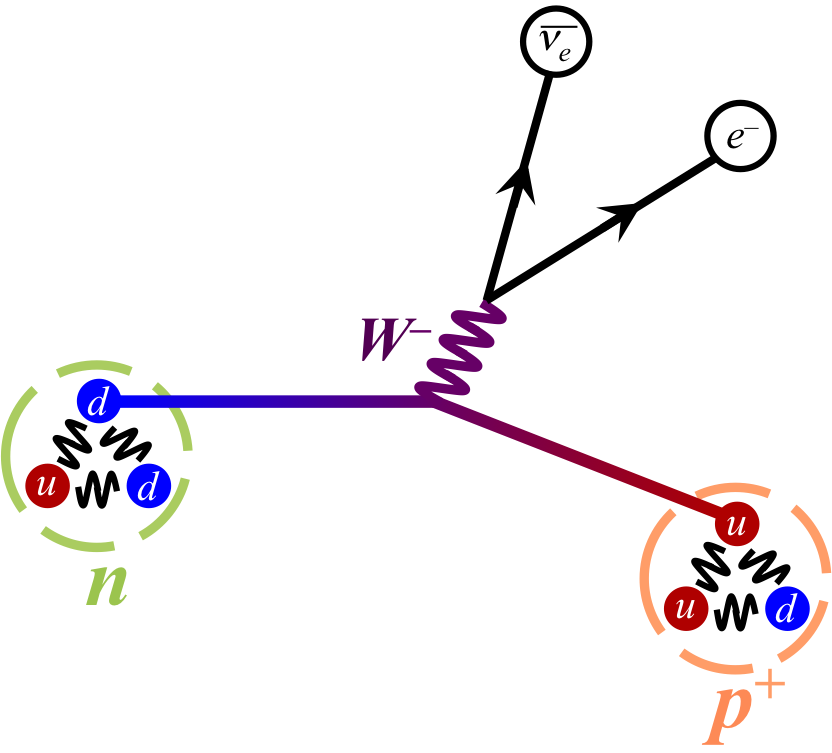
\includegraphics[width=0.5\columnwidth]{Neutrino/ntop.png}
\caption{Schematic space-time diagram representation of the weak interaction involved in the $\beta^{-}$ decay. Time flows from left to right. The sinusoidal lines are bosons: gluons in black, confining the quarks via the strong interaction; and the $W$ boson in purple. $p^{+}$ refers to a proton $^{1}_{1}\mathrm{H}^{+}$}
\label{fig:weakcurrent}
\end{center}
\end{figure}

In laymen terms, the weak force is the interaction involved whenever a quark alters its flavour. In Fig.~\ref{fig:weakcurrent}, one of the neutron's valence quarks' flavour switches from down (in blue) to up (in red) --- transmutting the composite particle from a neutron to a proton in the process --- the cost of which is the emission of a charged (here negatively charged) $W$ boson. The latter is short-lived and decays into an electron and an electron-flavoured antineutrino. The Feynman diagram in Fig.~\ref{fig:weakcurrent} illustrates the $\beta^{-}$ decay reaction described in Eq.~\ref{eq:beta_cont}. By reversing the charge, parity or time operators of one or several of the products or reactants involved, this Feynman diagram can also describe the electron capture and inverse $\beta$ decay:

\begin{equation}
\label{eq:three_reactions}
\left\{  
\begin{array}{rl}
^{1}_{0}n &\longrightarrow ^{1}_{1}\mathrm{H}^{+} + e^{-} + \bar{\nu}_e \\
e^{-} + ^{1}_{1}\mathrm{H}^{+} &\longrightarrow ^{1}_{0}n + \nu_e \\
\bar{\nu}_e + ^{1}_{1}\mathrm{H}^{+} &\longrightarrow ^{1}_{0}n + e^{+}
\end{array}
\right.
\end{equation}

In all cases, this basic description of the charged current weak interaction illustrates how a generic quark interacts non-elactically with a generic lepton.

\subsubsection{Lepton Flavours}

Neutrinos and antineutrinos can be produced by both the $W^{\pm}$ and $Z^0$ bosons:
\begin{equation}
\begin{array}{lcccr}
W^{+} \longrightarrow e^{+} + \nu_e & ~~~~~ & W^{-} \longrightarrow e^{-} + \bar{\nu}_e & ~~~~~ & Z \longrightarrow \nu_e + \bar{\nu}_e \\
\\
W^{+} \longrightarrow \mu^{+} + \nu_\mu & ~~~~~ & W^{-} \longrightarrow \mu^{-} + \bar{\nu}_\mu & ~~~~~ & Z \longrightarrow \nu_\mu + \bar{\nu}_\mu \\
\\
W^{+} \longrightarrow \tau^{+} + \nu_\tau & ~~~~~ & W^{-} \longrightarrow \tau^{-} + \bar{\nu}_\tau & ~~~~~ & Z \longrightarrow \nu_\tau + \bar{\nu}_\tau
\end{array}
\end{equation} \\ A neutrino's or antineutrino's lepton flavour is defined as that of the charged lepton with which it is interacting. The $W$ bosons can also decay into a quark anti-quark pair $q\bar{q}$. The $W$ decay channels are summarized in Fig.~\ref{fig:Wdecay}. Its decay width, of $\Delta m_W = 2.085 \pm 0.042~\mathrm{GeV}/c^2$ \citep{W_decay_width}, is proportional to the summed probability of all the possible aforementioned decay channels, and is consistent with $3$ lepton charges, hence a total of $3$ generations of leptons, either charged or neutral. In other words, if a fourth neutrino were to be discovered, it wouldn't have a lepton charge as it wouldn't interact with the $W$ bosons, hence making it insensitive to the weak interaction. \\

The particle discovered by Cowan, Reines and their collaborators is the electron flavoured antineutrino. In the early 1940s, an additional neutrino particle was hypothesized: the \textbf{neutretto}, which later became commonly known as the muon flavoured neutrino. It was discovered in 1962 by Leon Max Lederman, Melvin Schwartz and Jack Steinberger \citep{nu_mu_discovery}, who were awarded the 1988 physics Nobel prize. The third neutrino lepton flavor was hypothesized upon the discovery of the tau ($\tau^{-}$) lepton in a series of experiments at the Stanford Linear Accelerator Center (SLAC-LBL) from 1974 to 1977 \citep{tau_discovery}. The tau neutrino was discovered in 2000 by the Direct Observation of the Nu Tau (DONUT) collaboration \citep{nu_tau_discovery} at Chicago's Fermilab. \\

\begin{figure}
\begin{center}
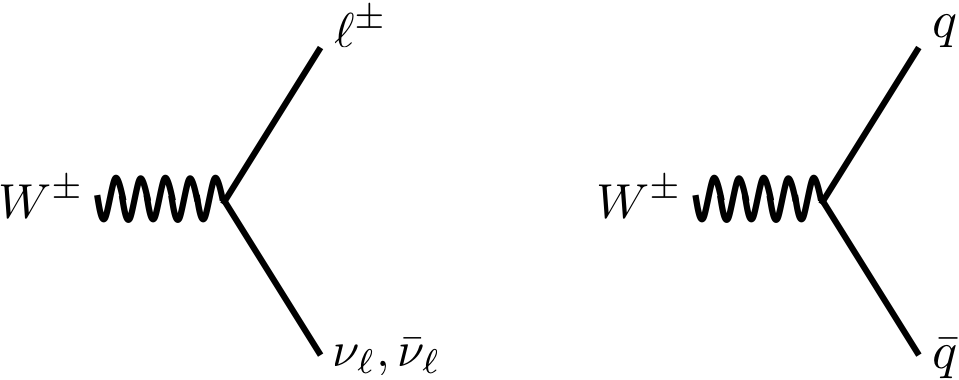
\includegraphics[width=0.5\columnwidth]{Neutrino/Wdecay.png}
\caption{\textbf{Left:} $W$ decay into a lepton pair (charged and neutral) $\ell \in \lbrace e, \mu, \tau \rbrace$. \textbf{Right:} $W$ decay into a quark anti-quark pair.}
\label{fig:Wdecay}
\end{center}
\end{figure}


\subsubsection{Helicity}


All particles have angular momentum, which for those described by quantum mechanics\footnote{quantum mechanics is often erroneously described as the theory which descibes small systems. What is implied by small is the characteristic length of the system. However, quantum mechanics can apply to large systems such as neutron stars, and can not apply to small systems such as a handful of gas molecules. In more exact terms, quantum mechanics applies to systems whose \textbf{action} is comparable to the Planck constant.} is the vector sum of its orbital momentum and its spin $\vec{j} = \vec{\ell} + \vec{s}$. Since the orbital momentum is orthogonal to the plane formed from the position and linear momentum, $\vec{\ell} = \vec{r} \times \vec{p}$, its component along $\vec{p}$ is zero. Helicity, defined as the projection of spin onto the direction of linear momentum,

\begin{equation}
\hat{h} = \vec{s} \cdot \frac{\vec{p}}{\vert \vert \vec{p} \vert \vert}
\end{equation} \\ is a conserved quantity. Since the spin's eigenvalues are discrete along an axis, so are those of the particle's helicity, which are $[\![ -s, +s ]\!]$ with $s$ the spin of the particle. As such, fermions with $s/\hbar=1/2$ can have $\pm 1$ helicity. Particles having positive (\textit{resp.} negative) helicity, \textit{i.e.} whose spin is aligned (\textit{resp.} opposed) to its linear momentum, are commonly refered to as being \textbf{right-handed} (\textit{resp.} \textbf{left-handed}). The choice of this nomenclature is motivated by the schematic in Fig.~\ref{fig:helicity}. \\
 
\begin{figure}
\begin{center}
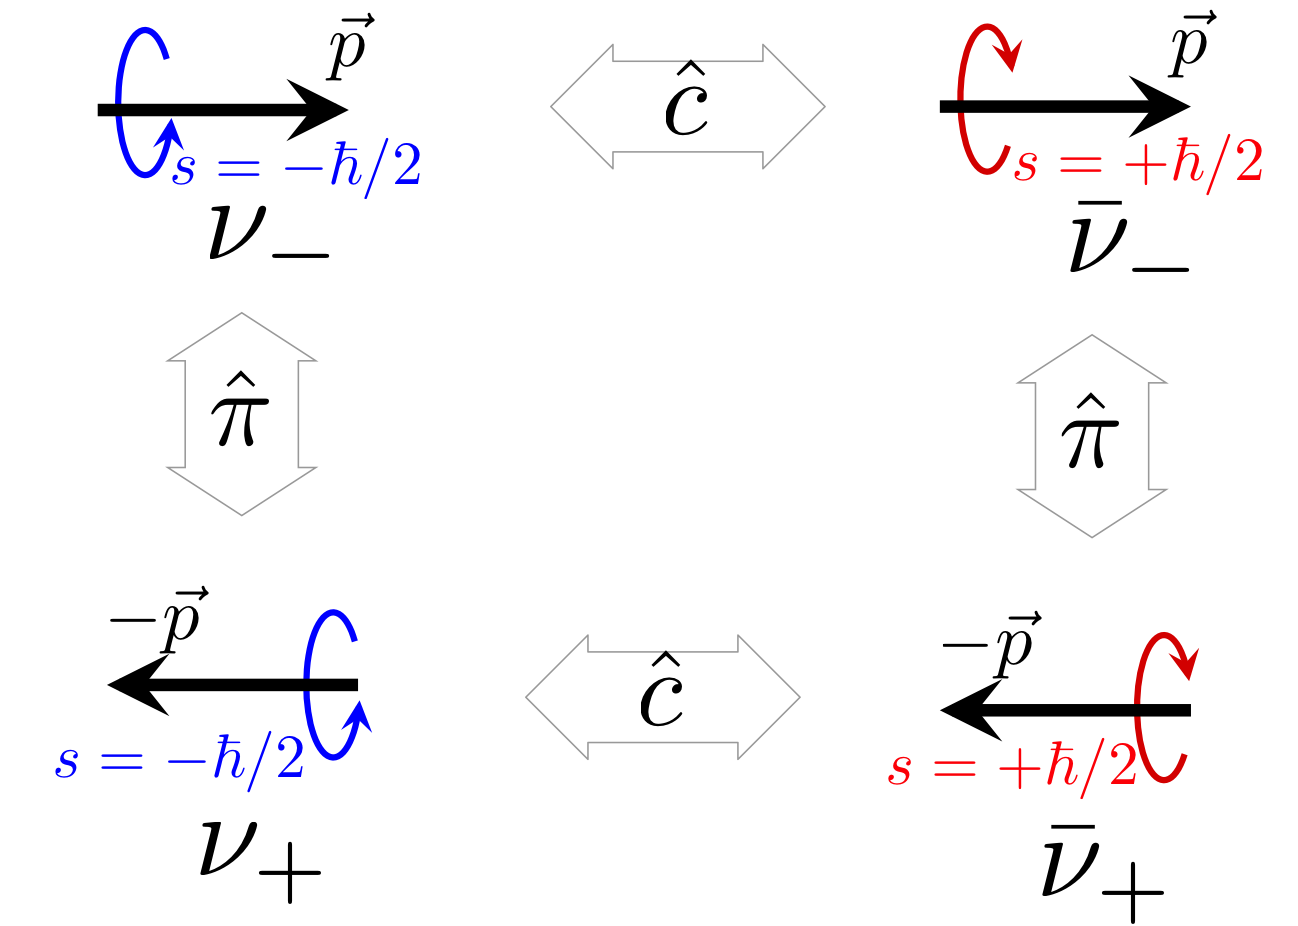
\includegraphics[width=0.75\columnwidth]{Neutrino/helicity.png}
\caption{Clockwise from top left: Left-handed neutrino, left-handed antineutrino, right-handed antineutrino and right-handed neutrino. The black arrows depict the particle's linear momentum. Its direction is inversed by the parity operator $\hat{\pi}$ applied from top to bottom row. The red and blue arrows depict the particle's spin. Its sign is inversed by the charge conjugation operator $\hat{c}$, applied from left to right columns. The $\pm$ subscipts denote the sign of the particle's helicity. The right or left handedness illustrates how the arrows materializing the spin of the particles wrap around the pointing direction of $\vec{p}$, as one's fingers wrap around the thumb. So far, only the negative helicity neutrino (top left) and positive helicity antineutrino (bottom right) are observed states in nature and predicted by the SM. The remaining two states are hypothetical and introduced in the $\nu$MSM in Sec.~\ref{sec:numsms}.}
\label{fig:helicity}
\end{center}
\end{figure}

A particle's linear momentum is relative to a reference frame, while its spin is invariant. Therefore, the particle's helicity, like its linear momentum, depends on the reference frame. Two observers, one moving slower and the other faster than a moving electron will disagree on the direction of its linear momentum with respect to their reference frame, and thus disagree on the electron's helicity sign. \\

In the SM, neutrinos are massless and therefore travel at the speed of light. As a consequence, there are no observers capable of travelling faster than the neutrino, hence only one of the two helicity signs is observed. Neutrinos appear to have intrinsically left-hand helicity. In the SM, the only right-handed neutral leptons are anti-neutrinos. Consequently, the weak interaction involving neutrinos or anti-neutrinos violates conservation of parity\footnote{the parity operator $\hat{\pi}$ mirrors the coordinates of a wavefunction, \textit{i.e.} $\hat{\pi} \left\vert \psi (\vec{r}) \right\rangle = \left\vert \psi (-\vec{r}) \right\rangle$}.  \\




\subsection{Why Neutrinos Are Interesting}

Neutrinos, despite completing our understanding of $\beta$ decay and other weak processes, are of particular interest in particle physics as they hint at the incompleteness of the Standard Model. The question whether neutrinos are a Dirac or Majorana particle remains to this day unanswered. If the latter is correct, which is plausible since they are electrically neutral, then that could resolve the issue of their left-handedness. If such is the case, then one would expect to observe neutrinoless $\beta$ decay processes, which haven't been confirmed as of today. \\

An antiparticle's wave function is the conjugate of its corresponding particle. In terms of the charge conjugation operator $\hat{c}$, $\left\vert \bar{\psi} \right\rangle = \hat{c} \left\vert \psi \right\rangle$. If this identity is applied to a neutrino, then its conjugate antineutrino would have the same helicity state. Since the left-handed  antineutrino state is currently unobserved in nature, one needs to apply the parity operator to the antineutrino's wave function, which reverse the linear momentum direction but conserves spin orientation, thereby reversing the helicity (see Fig.~\ref{fig:helicity}):

\begin{empheq}[box=\mymath]{equation}
\left\vert \bar{\nu} \right\rangle = \hat{c} \hat{\pi} \left\vert \nu \right\rangle
\end{empheq} \\ Although weak interactions don't conserve parity, its Hamiltonien $\hat{\mathcal{H}}$ commutes with $\hat{c}\hat{\pi}$ --- also called CP symmetry preservation --- since it is \textit{a priori} an invariant under this transformation. As recently as early August 2017, the Tokai to Kamioka (T2K) experiment has announced hints of a possible CP violation by neutrinos\footnote{\url{http://t2k-experiment.org/2017/08/t2k-2017-cpv/}}. If neutrinos indeed violate CP symmetry, they could provide a plausible explanation for the lepton (and baryon) asymmetry in the Universe. \\



On the astrophysical side, if detected in large enough quantities, they can serve as an alternative messenger from photons. The short range of their interaction with matter enable them to travel through dense zones unimpeded, but they also make their detection all the more challenging. This double-edged sword can nevertheless be useful in probing the Sun's core or the central zone of a supernova explosion, which produce massive quantities of neutrinos.\\


Provided neutrinos have non-zero mass, they could also constitute a candidate particle for dark matter. 
%\subsection{The Standard Model of Particle Physics}

%\subsection{Discovery of Neutrinos}

%\subsection{Neutrinos' Properties}

\clearpage